% \begin{frame}
%   \frametitle{Motivating latent dimensions: example data}
%   %% \framesubtitle{}

%   \begin{columns}
%     \begin{column}{6.5cm}
%       \begin{itemize}
%       \item Example: term-term matrix
%       \item V-Obj cooc's extracted from BNC
%         \begin{itemize}
%         \item targets = noun lemmas\\
%         \item features = verb lemmas
%         \end{itemize}
%       \item feature scaling: association scores (modified $\log$ Dice
%         coefficient)
%       \item $k=111$ nouns with $f \geq 20$\\
%         (must have non-zero row vectors)
%       \item $n=2$ dimensions: \emph{buy} and \emph{sell}
%       \end{itemize}
%     \end{column}
%     \begin{column}{4cm}
%       \begin{center}\footnotesize
%         \begin{tabular}{l|rr}
%           noun & \emph{buy} & \emph{sell} \\
%           \hline
%           \emph{bond}      &  0.28 &  0.77\\
%           \emph{cigarette} & -0.52 &  0.44\\
%           \emph{dress}     &  0.51 & -1.30\\
%           \emph{freehold}  & -0.01 & -0.08\\
%           \emph{land}      &  1.13 &  1.54\\
%           \emph{number}    & -1.05 & -1.02\\
%           \emph{per}       & -0.35 & -0.16\\
%           \emph{pub}       & -0.08 & -1.30\\
%           \emph{share}     &  1.92 &  1.99\\
%           \emph{system}    & -1.63 & -0.70
%         \end{tabular}
%       \end{center}
%     \end{column}
%   \end{columns}
% \end{frame}

% \begin{frame}[c]
%   \frametitle{Motivating latent dimensions \& subspace projection}
%   %% \framesubtitle{}
%   \begin{center}
%     \ungap[1]
%     \includegraphics[width=8cm]{img/3_buy_sell_labels_only}
%   \end{center}
% \end{frame}

\begin{frame}
  \frametitle{Motivating latent dimensions \& subspace projection}
  %% \framesubtitle{}

  \begin{itemize}
  \item The \h{latent property} of being a commodity is ``expressed''
    through associations with several verbs: \emph{sell}, \emph{buy},
    \emph{acquire}, \ldots
  \item Consequence: these DSM dimensions will be \h{correlated}
  \item[]
  \item Identify \h{latent dimension} by looking for strong correlations\\
    (or weaker correlations between large sets of features)%
  \item Projection into subspace $V$ of $k < n$ latent dimensions\\
    as a ``\h{noise reduction}'' technique \so \hh{LSA}
  \item Assumptions of this approach:
    \begin{itemize}
    \item ``latent'' distances in $V$ are semantically meaningful
    \item other ``residual'' dimensions represent chance co-occurrence
      patterns, often particular to the corpus underlying the DSM
    \end{itemize}
  \end{itemize}
\end{frame}

\begin{frame}[c]
  \frametitle{The latent ``commodity'' dimension}
  %% \framesubtitle{}
  \begin{center}
    \ungap[1]
    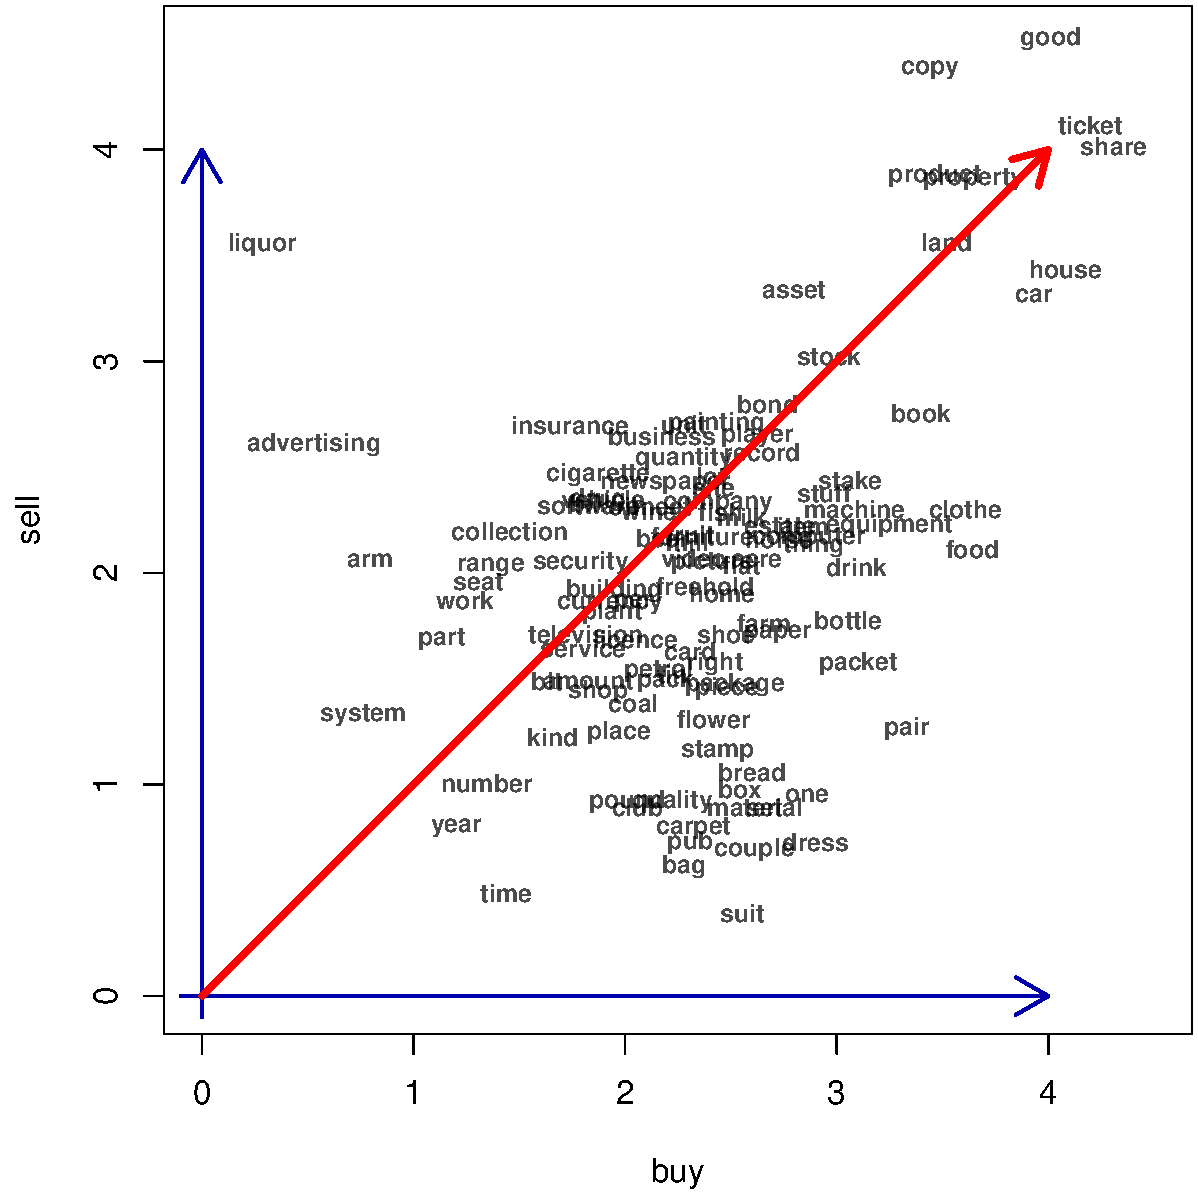
\includegraphics[width=8cm]{img/3_buy_sell_labels_latent}
  \end{center}
\end{frame}

%%% Local Variables: 
%%% mode: latex
%%% TeX-master: "../../workspace"
%%% End: 
